\documentclass[specification,annotation]{itmo-student-thesis}
% \documentclass[specification,annotation]{itmo-student-thesis}

%% Опции пакета:
%% - specification - если есть, генерируется задание, иначе не генерируется
%% - annotation - если есть, генерируется аннотация, иначе не генерируется
%% - times - делает все шрифтом Times New Roman, требует пакета pscyr.

%% Делает запятую в формулах более интеллектуальной, например:
%% $1,5x$ будет читаться как полтора икса, а не один запятая пять иксов.
%% Однако если написать $1, 5x$, то все будет как прежде.
\usepackage{icomma}

%% Данные пакеты необязательны к использованию в бакалаврских/магистерских
%% Они нужны для иллюстративных целей
%% Начало
% \usepackage{tikz}
% \usetikzlibrary{arrows}
% \usepackage{filecontents}
\urlstyle{sf}
\graphicspath{ {images/} }
\PassOptionsToPackage{hyphens}{url}

%% Конец

%% Указываем файл с библиографией.
% \addbibresource{bib/cryptobib-abbrev0.bib}
% \addbibresource{bib/cryptobib-crossref.bib}
\addbibresource{custom.bib}

\begin{document}

\studygroup{M3438}
\title{Тайм-трекинг пользовательских действий на распределенной блокчейн-сети}
\author{Волхов Михаил Александрович}{Волхов М.А.}
\supervisor{Штукенберг Дмитрий Григорьевич}{Штукенберг Д.Г.}{специалист}{тьютор кафедры КТ Университета ИТМО}
\publishyear{2017}
%% Дата выдачи задания. Можно не указывать, тогда надо будет заполнить от руки.
% \startdate{01}{сентября}{2016}
%% Срок сдачи студентом работы. Можно не указывать, тогда надо будет заполнить от руки.
% \finishdate{31}{мая}{2017}
%% Дата защиты. Можно не указывать, тогда надо будет заполнить от руки.
% \defencedate{15}{июня}{2015}

% \addconsultant{Йонн Мостовой}{без степени, без звания}

%% Задание и аннотация
%%% Техническое задание и исходные данные к работе
\technicalspec{Предложить дизайн системы для тайм-трекинга
  многопользовательских действий с помощью блокчейн-технологии.  }

%%% Содержание выпускной квалификационной работы (перечень подлежащих разработке вопросов)
\plannedcontents{
  \begin{enumerate}
  \item Постановка задачи и обзор предметной области.
  \item Анализ изменений базовой технологии (криптовалюты), связанный
    с разработкой.
  \item Разработка архитектуры.
  \end{enumerate}}

%Алгоритм должен поддерживать многопользовательские действия. Должна быть разрабтана формализация социальных контрактов и система оценки пользовательских действий на основании данных тайм-трекинга.

%%% Исходные материалы и пособия
\plannedsources{
  \begin{enumerate}
  \item Eli Ben-Sasson, Alessandro Chiesa, Christina Garman, Matthew Green, Ian Miers, Eran Tromer, Madars Virza, Zerocash: Decentralized Anonymous Payments from Bitcoin, proceedings of the IEEE Symposium on Security \& Privacy (Oakland) 2014, 459-474, IEEE, 2014;
  \item Aggelos Kiayias, Alexander Russell, Bernardo David, Roman Oliynykov, Ouroboros: A Provably Secure Proof-of-Stake Blockchain Protocol, 2017.
  \item Satoshi Nakamoto. Bitcoin: A peer-to-peer electronic cash system, http://bitcoin.org/bitcoin.pdf, 2008.
  \end{enumerate}
}

%%% Календарный план
\addstage{Ознакомление с имеющимися решениями в сфере тайм-трекинга}{02.2017}
\addstage{Ознакомление с практиками построения современных криптовалют}{02.2017}
\addstage{Реализация общего вида алгоритма}{03.2017}
\addstage{Написание пояснительной записки с проработанным формальным фреймворком}{04.2015}
\addstage{Доработка записки и доказательств}{05.2015}

%%% Цель исследования
\researchaim{Разработка тайм-трекинг системы с мультипользовательскими контрактами как надстройки над криптовалютой}

%%% Задачи, решаемые в ВКР
\researchtargets{\begin{enumerate}
  \item Соответствие алгоритма требованиям архитектуры блокчейн.
  \item Гибкий интерфейс: возможность реализации мобильного клиента для использования с алгоритмом.
  \item Формализация контрактной системы должна покрывать минимум повторяющиеся контракты с фиксированным временем в период.
  \item Алгоритм должен быть спроектирован так, чтобы не нарушать гарантий безопасности базовой системы.
\end{enumerate}}

%%% Использование современных пакетов компьютерных программ и технологий
\advancedtechnologyusage{Была использована система компьютерной
  верстки \LaTeX, программа для визуализации графов graphviz.}

%%% Краткая характеристика полученных результатов
\researchsummary{ В результате данной работы была разработана
  архитектура тайм-трекера, являющаяся надстройкой над протоколом
  криптовалюты Ouroboros. Решение имеет поддержку
  многопользовательских действий и контрактов. Также были
  проанализированы модификации Ouroboros, необходимые для построения
  решения. }

%%% Гранты, полученные при выполнении работы
\researchfunding{Грантов при выполнении работы получено не было.}

%%% Наличие публикаций и выступлений на конференциях по теме выпускной работы
\researchpublications{Данная работа не имеет публикаций.}

%% Эта команда генерирует титульный лист и аннотацию.
\maketitle{Бакалавр}

%% Оглавление
\tableofcontents

%% Макрос для введения. Совместим со старым стилевиком.
\startprefacepage

Решения, основанные на блокчейне, показывают возможность создания
распределенной сети, решающей конкретную проблему, одновременно не
требуя доверия к конкретным узлам сети и поддерживая стабильность
протокола. Блокчейн был применен в разных сферах проектирования
ПО. Особенно популярными стали решения в области криптовалют,
основанные на блокчейне, такие как Bitcoin \cite{bitcoin}, Ouroboros
\cite{ouroboros}. Также существуют системы для распределенного
хранения данных (storj \cite{wilkinson2014storj}, Permacoin
\cite{permacoin}), голосования (followmyvote\footnote{Follow my vote:
  \url{https://followmyvote.com/}}, bitcongress\footnote{BitCongress:
  \url{http://www.bitcongress.org/}}), идентификации пользователей,
реализация DNS протокола
(Namecoin \footnote{\url{https://wiki.namecoin.info/index.php?title=Domain_Name_Specification}})
и прочие \cite{swan2015blockchain}. Блокчейн -- это простое и
устойчивое решение для создания распределенной сети с большим
количеством узлов, что является ограничением BFT (byzantine fault
tolerant -- устойчивым к проблеме византийских генералов) алгоритмов
достижения консенсуса \cite{powbftquest}. Блокчейн-решения хорошо
масштабируются горизонтально и предоставляют базу для алгоритмов,
имеющих гарантии безопасности относительно различных атак.

Программное обеспечение для организации рабочего процесса и
тайм-трекинга на первый взгляд полностью противоположно продуктам,
основанным на блокчейне. Все рассматриваемые решения можно условно
поделить на две категории: органайзеры (google
calendar\footnote{Google calendar:
  \url{https://gsuite.google.com/learning-center/products/calendar/}},
remember the milk\footnote{Remember the milk: online to-do list and
  task management \url{https://www.rememberthemilk.com/tour/}}) и
тайм-трекеры (arbtt\footnote{Arbtt: completely automatic time tracker
  \url{https://arbtt.nomeata.de/#what}}, toggl\footnote{Toggl time
  tracker \& employee timesheet software
  \url{https://toggl.com/}}). Некоторые продукты совмещают в себе обе
функциональности: org-mode\footnote{Org-mode:
  \url{http://orgmode.org/}}, youtrack\footnote{ Youtrack:
  \url{https://www.jetbrains.com/youtrack/}}. Органайзеры оперируют в
терминах задач. Задачам можно присвоить различные временн\'{ы}е
атрибуты, вроде запланированного времени, чтобы не пропустить важную
встречу. Тайм-трекеры позволяют эффективно снимать статистику о том,
как пользователь тратит свое время. Анализ собранной статистики может
помочь найти проблемные места в организации жизнедеятельности
(например, выявлять и устранять прокрастинацию).

Однако, автору не известно ни одно решение, поддерживающее
мультипользовательский тайм-трекинг. Под этим термином подразумевается
возможность хранения не только информации о том, что группа
пользователей совместно участвовала в какой-то деятельности, но и
подтверждение этой информации от каждого участника. Эта идея
продолжается на мультипользовательские контракты. Если сервис имеет
достаточно знаний о том, какие группы пользователей должны тратить
время совместно на установленные задачи и в каком объеме, то оценка
таких соглашений может быть автоматизирована, если известны данные о
тайм-трекинге.

Блокчейн и криптовалюты предлагают прямое решение. Во-первых, идея
мультипользовательского тайм-трекинга близка к идее
мультипользовательских транзакций. Во-вторых, большинство криптовалют
реализуют в том или ином виде фреймворк для скриптинга, который
позволяет выполнять произвольные вычисления с данными на блокчейне,
что может быть эффективно использовано для распределения очков
рейтинга в рамках контракта. Необходимые свойства представлены, к
примеру, в Ethereum \cite{ethereum} (смарт-контракты,
децентрализованные автономные организации), Hawk \cite{kosba2016hawk}
(анонимные смарт-контракты с использованием
zk-доказательств). В-третьих, высокий рейтинг пользователей
свидетельствует о их компетентности в вопросе
договоренностей. Блокчейн представляет эффективный способ хранения
псевдо-публичной информации и дает возможности гибко настроить
механизм публикации таких данных.

Для большей наглядности того, как могут быть применена система с
поддержкой мультипользовательских контрактов и транзакций, приведем
два примера:

\begin{enumerate}
  \item Модифицированный семейный спор. Бессрочный контракт периодом в
    две недели предполагает, что на активность ``театр'' будет
    потрачено как минимум 3 часа в одной транзакции, а на активность
    ``футбол'' будет потрачено не менее четырех (в рамках
    периода). При этом контракт обязывает обоих партнеров участвовать
    в каждой из этих активностей. Придя на мероприятие, супруги (с
    помощью мобильного приложения) отмечают начало и тип действия, а
    по окончании каждый подтверждает эту информацию с помощью своего
    публичного ключа (опять-таки, через интерфейс мобильного
    приложения). По истечении недели умный контракт распределяет
    супругам очки рейтинга в зависимости от того, как были
    удовлетворены нужды каждого партнера. Ни один из участников не в
    силах самостоятельно подделать информацию о совместном
    времяпровождении. Поскольку партнеры пытаются максимизировать свой
    рейтинг, их стратегия должна быть построена так, чтобы избегать
    посещения мероприятий в одиночку. Любой из партнеров может
    провести псевдо-публичный аудит этой информации стороннему лицу,
    подтвердив свою способность следовать семейным
    договоренностям. Схема хорошо обобщается на полиаморические
    отношения.
  \item Фриланс биржа. Компания, которая хостит сайт для фрилансеров,
    разворачивает локальный мультипользовательский тайм-трекер для
    использования в связке с функционалом сайта. Заказчик и
    исполнитель, оформляя контракт через сайт, создают скрипт-контракт
    в блокчейне. Они договариваются на 40 часов еженедельной работы в
    течение двух месяцев и на минимум два часовых митинга в течение
    каждой недели. Исполнитель отмечает свою рабочую деятельность с
    помощью интерфейса сайта и просит заказчика подтвердить транзакцию
    в конце дня, предоставляя ему сводку выполненных задач за
    день. Еженедельные митинги трекаются с обеих сторон. В случае
    невыполнения требований исполнитель теряет рейтинг, который
    привязан к его аккаунту.
\end{enumerate}

%% Начало содержательной части.
\chapter{Обзор предметной области}

\section{Децентрализованные платежные системы}

Биткоин -- первая распределенная платежная система, получившая
значительную популярность. Среди других подобных решений, биткоин
занимает 62\% всей рыночной капитализации\footnote{По данным
  \url{https://coinmarketcap.com/} на 28.04.2017}. Блокчейн-технология
для распределенного хранения состояния и вероятностный алгоритм PoW
(proof-of-work, дословно ``доказательство выполнения работы'') стали
идеальной комбинацией, которая и привела к его широкому
распространению. Традиционно децентрализованная платежные система,
использующая криптографические методы для построения алгоритма
консенсуса, называются {\it криптовалютой}. Существует много других
решений в сфере криптовалют, из которых значительная часть также
используют блокчейн и PoW.

\subsection{Пользователи, счета и транзакции}

Криптовалюта -- это система, позволяющая ассоциировать {\it адреса} со
средствами на нем, а также переводить эти средства с одного адреса на
другой с помощью {\it транзакций}. Пользователь криптовалюты может
иметь несколько адресов. Каждый адрес ассоциируется с публичным ключом
$Pk$, секретной компонентой $Sk$ которого владеет пользователь. В
качестве адреса чаще всего берется криптографический хэш $H(Pk)$, где
размерность хэш-пространства $H$ удобна для представления адреса
(меньше, чем размер самого $Pk$). Тут и далее публичный ключ и адрес
будут использоваться взаимозаменяемо, если это не вызывает
неоднозначности.

Транзакция $Tx$ состоит из входов $txIn$ и выходов $txOut$. Существует
два подхода к реализации транзакций: использующие балансы или
свободные выходы транзакций. Балансная реализация сопоставляет
пользователя с единственным числом -- его балансом. В таком случае
достаточно принять $txIn = \{AddrIn_i,\ a_i\}_{i=1}^n, \ txOut =
\{AddrOut_j,\ b_j\}_{j=1}^m$, где $a_i, b_j \in \mathbb{N}$ -- объем
переводимых средств. Более популярным является подход со свободными
выходами транзакций (unspent transaction outputs). Каждый элемент
$txIn$ представляется как $txout = (H(tx), i), i \in \mathbb{N}$ --
выход номер $i$ в транзакции с хэшем $H(tx)$. Этот подход более
эффективен с точки зрения объема транзакции, а также решает проблему
двойного расходования средств (double spending или replay attack):
каждая транзакция уникальная и не может попасть в блокчейн
дважды. Второй подход является более частным и может быть сведен к
первому: узел сети с помощью информации из блокчейна может получить
$a_i$ по $txout$. Подход с балансами будет использоваться для
формального описания транзакции далее.

Перед тем, как транзакция попадет в блок, она должна быть
пройти валидацию. Валидация транзакции состоит из двух этапов: проверки
балансов и проверки доказательства транзакции. Первая проверка
вычисляет разницу между входами и выходами транзакции $\Delta =
\sum_{i=1}^n{a_i} - \sum_{j=1}^m{b_j}$ и успешна только если $\Delta
\geq 0$. Пользователь, отсылая транзакцию в сеть, прикладывает к ней
{\it доказательство транзакции} (witness). Доказательство
содержит в себе подпись $\sigma_{Sk_i}(Tx)$ для каждого адреса
$Pk_i \in txIn$. Вторая проверка успешна только если
каждая подпись $\sigma_i$ корректна.

\subsection{Блокчейн}

Блокчейн -- решение для поддержки общего состояния узлов в сети,
обеспечивающее открытость (любой узел может присоединиться), полную
децентрализацию и отличное горизонтальное
масштабирование. Блокчейн/PoW решения обычно противопоставляются BFT
алгоритмам репликации состояния. Этот дуализм порождает компромиссную
модель, описанную в \cite{powbftquest}: в частности, BFT алгоритмы
обеспечивают большую пропускную способность и производительность.

Формально блокчейн представляет собой последовательность {\it блоков}
$B_1 \ldots B_n$, где $n$ -- текущая {\it сложность} цепи. Каждый блок
$B_i$ состоит из заголовка и тела. Тело блока содержит в себе
множество транзакций $Txs$. Заголовок в общем случае состоит из
публичного ключа {\it эмитента блока} $BPk$, хэш предыдущего блока в
цепи $H(B_{i-1})$, информации удостоверяющей тело (дерево меркла,
построенное на $Txs$), а также подпись всех вышеперечисленных полей
заголовка $\sigma_{BSk}(B)$.

Алгоритм PoW основывается на вычислительной сложности задачи. В
биткоине, это нахождение значения криптографической хэш-функции в
заданном интервале хэш-пространства. Эмитенту предлагается подобрать
такой $nonce$, что $H(nonce || H(B_{i-1})) < d$, где $d$ -- параметр
сложности. Участники сети стохастически перебирают $nonce$ до тех пор,
пока условие не будет выполнено, а затем добавляют $nonce$ внутрь
заголовка блока и отправляют его в сеть. Другие узлы сети проверяют,
что условие выполнено и принимают блок. В случае, если несколько
блоков имеют общих родителей, узел сети выбирает основной цепью самую
ту, которая имеет максимальную сложность. Процесс подбора значения
называется {\it майнингом}.

Существуют концептуально другие алгоритмы достижения консенсуса в
блокчейне. Так, например, Permacoin \cite{permacoin} предлагает схему,
основанную на доказательстве владения данными (Proof of Space или
Proof of capacity) -- пользователи, хранящие больше данных, имеют
больший шанс выпустить блок. Тем не менее, более популярным подходом
является доказательство владения средствами (Proof of Stake, PoS),
реализованный в ряде криптовалют: Nxt \cite{nxt}, Peercoin
\cite{king2012ppcoin}, Ouroboros \cite{ouroboros}, Blackcoin. Выбор
эмитента блока производится заранее пропорционально {\it стейку}
пользователя. Стейком является суммарное количество средств на счету
пользователя (или его часть, в nxt в стейк не входят средства,
полученные ранее, чем некоторый установленный интервал времени). PoS
алгоритмы элиминируют необходимость траты вычислительных ресурсов в
PoW алгоритмах (связанной с высоким энергопотреблением), поскольку
выбор лидера детерминирован.

\section{Ouroboros}

Ouroboros \cite{ouroboros} это первый протокол криптовалюты,
основанный на схеме PoS, имеющий доказанные гарантии безопасности
относительно условий стабильности цепи. Выбор этого протокола
обоснован несколькими ключевыми факторами. Во-первых, подход PoS
превосходит PoW решения как в защите от атак (selfish mining, bribery
attacks), так и в экономии вычислительных ресурсов. Остальные подходы
не являются достаточно формальными и популярными одновременно и так
или иначе тратят избыток физического ресурса. Во-вторых, Ouroboros
основан на идее слоттинга -- разбиения времени на слоты одинаковой
длительности. Таким образом, блоки выпускаются в фиксированный период
времени. Это свойство не выполняется в PoW решениях, где разница между
выпущенными блоками вероятностна, поскольку зависит от сложности
выпуска блока -- переменной, которая в общем случае меняется со
временем. Ресурс BlockchainInfo \footnote{Онлайн браузер блокчейна
  биткоина: \url{https://blockchain.info/}} предоставляет возможность
удостовериться, что реальное время выпуска блока в биткоин варьируется
от 1 до более чем 30 минут. Единственная на момент написания
реализация протокола называется Cardano
SL\footnote{\url{https://github.com/input-output-hk/cardano-sl}}.

\subsection{Общая модель протокола}

Эта подсекция описывает общую модель протокола Ouroboros.

\subsubsection{Слоттинг и параметры безопасности}

Протокол фиксирует следующие публично известные константы,
используемые для слоттинга: $startT, slotT, k, epochK$. $startT$ --
метка времени (в POSIX миллисекундах), означающая время начала работы
протокола. $slotT$ -- время одного слота в миллисекундах. $k$ это
константа безопасности, означающая количество последних неустойчивых
блоков в цепи. $epochK$ является множителем $k$, задающий эпоху. Для
удобства в дальнейшем введем еще одну переменную: $epochSlots = epochK
\times k$.

Слот -- это монотонно возрастающая функция от текущего времени
$currentT$, которая вычисляется как $getSlot(t) = (t - startT) /
slotT$, где все переменные имеют одну размерность (например,
миллисекунды). Длина слота $slotT$ должна быть больше ожидаемой
задержки на доставку среднего сообщения протокола.  Слот $j$
принадлежит эпохе $i$, если $i = \lfloor j / epochSlots \rfloor$.

Параметр безопасности $k$ определяет постоянство (persistence)
системы. Транзакция считается стабильной, если ее позиция в общей цепи
глубже, чем последние $k$ блоков.

\subsubsection{Свойства цепи блоков транзакций}

Блокчейн Ouroboros'а спроектирован в манере близкой к большинству
реализаций, в том числе к блокчейну биткоина. В отличие от
блокчейна биткоина, блоки Ouroboros'а делятся на два типа: главные
блоки и генезис блоки. Каждый главный блок имеет соответствующий
слот. Каждый (прошедший) слот имеет один соответствующий ему главный
блок, или не имеет вовсе.

Генезис блок содержит информацию о слот лидерах. Лидер слота это
участник сети (имеющий достаточную долю средств с точки зрения
блокчейна), который единственно уполномочен выпустить блок в
конкретный слот. В течение каждой эпохи алгоритм, называющийся SSC
(shared seed calculation, описан в следующей подсекции), собирает
случайные данные для формирования сида, который детерминировано
определяет слот лидеров следующей эпохи. Список слот лидеров и сид --
все, что находится в теле генезисного блока. Заголовок схож с
заголовком главного блока -- он содержит в себе доказательство данных
тела и эпоху. Генезис блоки выпускаются участниками сети независимо и
равны при условии того, что участники видят один и тот же префикс
блокчейна.

Главные блоки несут основную функциональность транзакционного журнала
и схожи с блоками, описанными в первой главе. Тело главного блока
содержит список транзакций, данные о SSC и другую относительно
объемную информацию (из механизмов делегации и системы обновлений, не
покрытых в этом описании). Заголовок содержит следующие поля:

\begin{enumerate}
\item Доказательство данных тела: дататайп, содержащий информацию,
  необходимую для того, чтобы авторизовать тело блока (дерево меркла
  поверх каждой компоненты тела).
\item Данные консенсуса: текущая эпоха и слот, сложность (высота
  текущего блока в общей цепи), публичный ключ лидера слота, подпись
  блока (заголовка, публичным ключом лидера слота).
\end{enumerate}

\subsubsection{SSC}

Ouroboros предлагает использовать вариант протокола конфиденциального
вычисления (multi-party computation, MPC) для вычисления равномерно
случайной строки, которая будет использована в процессе выбора
лидеров. Эта часть протокола называется SSC (shared seed calculation).

Коммитментом от случайной строки $r$ и сообщения $m$ является такое
сообщение $c = Com(r,m)$, что для парной функции раскрытия $o =
Open(r,m)$ само $o$ является доказательством того, что $m$ --
сообщение внутри $c$. В то же время $c$ сам по себе не раскрывает
никакой информации о $m$.

Участвовать в протоколе SSC могут только те пользователи, которые
имеют достаточно средств (выше установленного порога $sscThreshold$)
по состоянию на конец предыдущей эпохи. Каждая эпоха делится на три
фазы по: фаза коммитментов (первые $2k$ слотов), фаза раскрытий (слоты
$[4k, 6k-1]$) и фаза восстановления (слоты $[8k, 10k-1]$). В
первую фазу участники SSC рассылают в сеть коммитменты. Во вторую фазу
они раскрывают свои коммитменты, отправляя раскрытия коммитментов,
сделанных ранее. Третья фаза необходима для восстановления
коммитментов при условии недостаточного количества раскрытий. Для
этого используется протокол VSS (verifiable secret sharing)
\cite{feldman1987practical}.

Все данные SSC хранятся в телах главных блоков.

\subsection{Система поощрений}

Система поощрений является набором правил, которые стимулируют
участников протокола принимать участие в выпуске блоков и SSC с
помощью присвоения им награды.

Для того, чтобы мотивировать участников принимать транзакции, каждому
слоту присваивается фиксированное количество эндорсеров. Задача
эндорсера состоит в том, чтобы собирать транзакции в сети. Лидер слота
получает подписанные данные от эндорсеров, объединяет их и кладет эти
данные в блок. Каждый участник сети может установить соответствие
между транзакциями и эндорсерами, от которых они были получены.

В систему также вводится понятие комиссии транзакции. Проверка
транзакции на валидность допускает ненулевую разницу между суммой
выходов и входов транзакции. Это значение и называется комиссией. Все
комиссии за эпоху $e$ суммируются, получая значение $S$. Протокол
предлагает равномерное распределение $S$ среди лидеров слота и
эндорсеров: участник $U$ может претендовать на долю $\frac{m S}{n}$, где
$m$ это количество раз которое он был лидером или эндорсером за эпоху
$e$, а $n$ суммарное число лидеров и эндорсеров в эту эпоху. $U$
получает деньги, отправляя себе транзакцию с указанной суммой в эпоху
$e+1$.

Утверждается, что представленная стратегия распределения награды
соответствует приближенному равновесию по Нэшу, то есть любой участник
протокола, отклоняющийся от него, получает не более $1 + \epsilon$ той
награды, которую он бы точно получил, придерживаясь протокола.

\section{Улучшения и дополнительная функциональность}

Существует множество дополнительных модификаций, широко поддерживаемых
криптовалютами. Некоторые из них автономны, но существенная часть была
впервые предложена в биткоине и специфицирована в
BIP \footnote{Bitcoin wiki: BIP
\url{https://en.bitcoin.it/wiki/Bitcoin_Improvement_Proposals}}
(bitcoin improvement proposals), а затем портирована на другие
решения.

\subsection{Скриптинг и P2SH}

Скриптинг или P2SH (pay-to-script-hash, дословно ``перевод на хэш
скрипта'') -- модификация криптовалюты, позволяющая пользователям
создавать адреса с гибкими, настраиваемыми условиями снятия
денег. Поддерживается многими решениями: Ethereum, Nxt, в биткоине
стандартизирована под
BIP16 \footnote{\url{https://github.com/bitcoin/bips/blob/master/bip-0016.mediawiki}}
\cite{seijas2016scripting}. Данная часть опишет фреймворк в общем
виде, придерживаясь терминов определенных в Plutus \cite{plutus} --
скриптового языка Cardano SL.

Протокол криптовалюты определяет поддерживаемый скриптовый язык. Он
может быть как тьюринг-полным (Plutus в CSL; байткод Ethereum в
который компилируются высокоуровневые Solidity \cite{solidity} и
Serpent \cite{serpent}), так и неполным (биткоин использует стековый
язык Script, являющийся модификацией Форта
\cite{bitcoinwikiscript}). Пользователь создает скрипт-валидатор,
который принимает один аргумент произвольного типа и возвращает
результат, интерпретируемый как булевое значение. Валидатор может быть
захеширован и использован как публичный адрес криптовалюты. Любой
пользователь может перевести средства на этот адрес. Для того, чтобы
перевести деньги с этого адреса, к доказательству транзакции должна
быть приложена пара из двух скриптов. Один из них -- валидатор, хэш
которого должен совпадать с адресом, с которого списываются
средства. Второй -- ридимер, генерирует входные данные для
валидатора. Чтобы проверить валидность траты входа транзакции, нужно
сгенерировать аргументы ридимером, передать их валидатору и
удостовериться, что последний вернул $True$.

Основная реализация протокола Ouroboros (Cardano
SL\footnote{https://github.com/input-output-hk/cardano-sl}) использует
скриптовый язык Plutus. Это функциональный тьюринг-полный язык со
строгой типизацией, схожий с Haskell. Скрипт-валидатор в Plutus имеет
типовую сигнатуру \lstinline|validator :: A -> Comp B|, где
\lstinline|Comp| это встроенный дататайп, изоморфный $Maybe$ с
точностью до инстанса класса монады. Он имеет два конструктора:
\lstinline|success :: B -> Comp B| и \lstinline|failure :: Comp B|.
Скрипт-ридимер в Plutus имеет тип \lstinline|Comp A|. Несложно видеть,
что поскольку $Comp$ является монадой, то проверка возможности
потратить инпут есть \lstinline|redeemer >>= validator|. Стоит
отметить, что несмотря на то, что возвращаемое значение валидатора --
это \lstinline|Comp a|, алгоритм валидации не проверяет значение
внутри конструктора, а лишь удостоверяется, что значение не является
\lstinline|failure|.

Приведем пример тривиального валидатора и ридимера.

\begin{lstlisting}[float=!h,caption={Пример пары валидатор/ридимер на Plutus}]
data Foo = { Foo | Bar }

validator : Foo -> Comp Unit {
    validator x = case x of {
        Foo  -> success MkUnit ;
        Bar  -> failure } }

redeemer : Comp Int {
    redeemer = success Foo }
\end{lstlisting}

Plutus имеет стандартную библиотеку, которая предоставляет базовые
типы данных и функции: обертки $Either$ и $Maybe$, списки и различные
предикаты. Также существует поддержка для добавления встроенных
функций. Встроенные функции могут использовать ресурсы узла сети. С
помощью них валидатор может, например, достать UTXO, относящееся к
конкретному блоку или периоду блокчейна. Фреймворк достаточно гибок
для реализации сложных операций валидации.

\subsection{Цветные монеты}

Цветные монеты (colored coins) это расширение криптовалюты,
позволяющее поддерживать разные типы сбережений. К значению ресурса
добавляется специальный тег, который называется цветом. Цветные
моменты были изначально стандартизированы и реализованы как настройка
над биткоином в стандарте
EPOBC\footnote{\url{https://github.com/chromaway/ngcccbase/wiki/EPOBC_simple}}
в 2012. В настоящий момент существуют еще несколько иных решений:
стандарт OAP \footnote{Open Assets Protocol
  \url{https://github.com/OpenAssets/open-assets-protocol/blob/master/specification.mediawiki}},
Coinspark\footnote{\url{http://coinspark.org/}} и
Colu\footnote{\url{https://www.colu.com/}}. Существуют виртуальные
кошельки, поддерживающие несколько стандартов
одновременно\footnote{ChromaWallet поддерживает OAP и OPOBC
  \url{http://chromawallet.com/}}. Стоит отметить, что все
перечисленные стандарты используют метаданные транзакций в биткоине
для передачи информации о цвете, а не изменяют протокол напрямую (что
привело бы к форку). Тем не менее, поддержка стандарта с изменением
протокола может быть сделана проще и эффективнее.

С интеграцией цветных монет связано несколько дополнительных
задач. Во-первых, изменяется логика валидации транзакции. Если раньше
достаточным условием было проверить, что сумма выходов не превосходит
сумму входов, то с цветными монетами существует несколько
подходов. Первый предлагает запрет на транзакции, ``красящие'' монеты
-- то есть изменяющие цвет в транзакции. В этом случае валидация
транзакции сводится к валидации сужений транзакций до каждого
цвета. Этот подход реализован во всех упомянутых
стандартах. Во-вторых, изменяется логика эмиссии ресурсов. OAP
предоставляет возможность производить эмиссию активов, удостоверяя
эмитента отдельным секретным ключом. Вместо возможности производить
чистую эмиссию можно предложить решение с покраской монет --
транзакция может менять тег средств, если она удовлетворяет правилам
покраски. Этот подход был применен при реализации цветных монет в
криптовалюте RSCoin\footnote{Репозиторий RSCoin на github:
  \url{https://github.com/input-output-hk/rscoin-haskell}}
\cite{danezis2015centrally}: монеты цвета $0$ могли быть покрашены в
цвет $i \neq 0$ (единственное правило перекраски). EPOBC решает
проблему похожим образом, разрешая перевод базовых монет (монет
базовой криптовалюты) в любой другой цвет.

\subsection{Иерархический детерминированный кошелек}

Дополнение к протоколу биткоина под названием HD кошелек (Hierarchical
Deterministic Wallets) было предложено в рамках BIP32 \cite{hdwallets}
и предлагает расширение схемы подписей secp256k \cite{sec20002},
решающее проблему дублирования секретных ключей на разных устройствах.

Пара ключей $Pk$ и $Sk$ (32 байта каждый) расширяются 32 байтами
энтропии $c$, которая называется кодом цепи (chain code), результируя
в пару расширенных ключей $Pke = (Pk, c)$ и $Ske = (Sk, c)$ по 64 байт
каждый. Затем вводятся две ключевые функции:

\begin{enumerate}
\item $CKDpriv : (Ske, i) \rightarrow Ske$. Принимает на вход расширенный
  секретный ключ $Ske$, целое число $i$ в интервале $[0, 2^{32})$ и
  возвращает расширенный секретный ключ
\item $CKDpub : (Pke, i) \rightarrow Maybe Pke$. Если $i \geq 2^{31}$, функция
  возвращает $Nothing$. Это расширение называется харденингом
  (hardening), запрещая выводить половину интервала публичных дочерних
  ключей. Если $i < 2^{31}$, возвращает расширенный публичный ключ.
\end{enumerate}

Функции $CKDpriv$ и $CKDpub$ построены таким образом, что каждая
расширенная пара $(Ske,Pke)$, полученная с их помощью для одного $i$,
является валидной парой секретный-публичный ключ. Возможность выводить
ключи в любом другом направлении (родительские из дочерних, секретные
из публичных) отсутствует.

Cardano SL использует схему цифровых подписей Ed25519
\cite{bernstein2012high} и модифицированную версию HD ключей, описанную
в \cite{ed25519hd}. Тем не менее, они взаимозаменяемы с точностью до
размерности ключей, функционала и представленного
интерфейса. Расширенные HD ключи/адреса являются основными с точки
зрения большинства алгоритмов (только обладатель публичного HD ключа
может быть лидером слота и т.д.).

\chapterconclusion

В данной части был проведен обзор предметной области, описаны решения
и алгоритмы, необходимые для построения функциональности тайм-трекинга
поверх криптовалюты.

\chapter{Описание алгоритма}

\section{Интеграция цветных монет}

Поскольку данная работа предлагает изменение протокола Ouroboros без
поддержки обратной совместимости, поддержка цветных монет существенно
упрощается, поскольку не требует надстраивания (например, через
метаданные транзакции). Эта секция описывает различные нюансы и детали
реализации.

\subsection{Граф конвертации цветов и валидация транзакций}

Воспользуемся схемой покраски монет, не прибегая к возможности эмиссии
активов нового цвета. Все монеты конвертируются один к одному.

\begin{definition}
Пусть $Col$ -- конечное множество элементов (цветов). Тогда (цветной)
монетой называется пара из целого номинала и цвета: $coin = (n,c), \ n
\in \mathbb{N}, \ c \in Col$.
\end{definition}

Сумма по цвету $\sum_c{Coins} = (\sum_{y \in F}{y}, c), \ F = \{y \mid
(y,c) \in Coins\}$ складывает номиналы отфильтрованных монет
указанного цвета $c$. Бесцветная сумма $\sum_{i=1}^n{coin_i} =
\sum_{i=1}^n{n_i}$ складывает только номиналы. Спектр множества монет
есть все цвета входящие в множество монет $\sigma(Coins) = \{c \mid
(n,c) \in Coins\}$. Также определим функционал $MergeC(C) = \{(c,n)
\mid c \in \sigma(C), \ n = \sum_c(C)\}$, оставляющий по одной монете
каждого цвета в множестве.

\begin{definition}
Граф конвертации цветов $G_c = (V,E)$ это ориентированный граф без
кратных ребер, в котором $V = Col$, а множество ребер $E$ содержит в
себе петлю для каждой $v \in V$. Ребро $e \in E$ называется правилом
конвертации цвета.
\end{definition}

Граф конвертации цветов удовлетворяет реальной модели обмена
ресурсов. $Col$ есть множество возможных тегов монет, ребро $uv \in
G_c$ представляет собой возможность перевести монеты цвета $u$ в
монеты цвета $v$. Необходимость петель исходит из ситуации обычного
одноцветного перевода средств. Граф конвертации в системе с одним
цветом монеты имеет одну вершину и одну петлю.

\begin{definition}
Транзакция $Tx$ -- это пара из входов и выходов $(txIn, txOut)$,
являющихся списками монет. Спектр транзакции $\sigma(Tx) = \sigma(txIn
\cup txOut)$. Сужение транзакции на цвет $Tx_c = (\sum_c{txIn},
\sum_c{txOut})$ есть пара балансов по этому цвету на входе и на выходе
транзакции.
\end{definition}

Правило валидации транзакции $Validate(Tx)$ должно соответствовать
двум требованиям:
\begin{itemize}
\item Сумма входов не меньше суммы выходов: $\sum(txIn) \geq \sum(txOut)$
\item Покраска монет соответствует графу конвертации цветов $G_c$.
\end{itemize}

В то время, как проверка первого свойства производится тривиально,
второе требует более тщательного рассмотрения. Предположим, что в
случае, если первая проверка показала $\Delta = \sum(txIn) -
\sum(txOut) \geq 0$, то добавим $(\Delta, basec)$ в $txOut$, где
$basec \in Col$ -- выделенный цвет. В следующей главе будет показано
практическая польза этого подхода. Поэтому отсюда и далее полагаем
$\Delta = 0$ для рассматриваемой $Tx$.

Пусть $txIn_m = MergeC(txIn)$. Выразим формально второе требование:
\begin{align*}
  \exists H = \ &\bigsqcup_{i=1}^s{H_i}. \ MergeC(H) = txIn_m \ \wedge \nonumber \\
                &\forall (n_{out},c_{out}) \in txOut . \ \exists i . \ H_i = (n_{out},c_{in}) \wedge c_{in}c_{out} \in G_c \label{eq:1}
\end{align*}

То есть существует такой способ разбить входы $txIn$ на $H_i$ что для
каждого элемента выхода найдется соответствующий $H_i$ совпадающий по
номиналу и соответствующий условию покраски. Отметим, что мы разрешаем
только один переход по ребру $G_c$ для каждой транзакции. В случае,
если реализация должна допускать транзитивную покраску в рамках одной
транзакции, следует использовать транзитивное замыкание $G_c^{+}$
вместо $G_c$.

Покажем, что проверка этого условия сводится к решению задачи о
максимальном потоке в графе. Пусть $D$ -- ориентированный граф,
построенный из $txIn$, $txOut$ и $G_c$ следующим образом. Пусть $E_e =
\{e_i\}_{i=1}^n = \sigma(txIn),\ E_x = \{x_j\}_{j=1}^m =
\sigma(txOut)$. Тогда определим множество вершин $V = \{s, t\} \cup
E_e \cup E_x$. Множество ребер $E = \{se_i\}_{i=1}^n \cup
\{x_jt\}_{j=1}^m \cup \{(e_i,x_j) \mid (e_i,x_j) \in G_c\}$. Ввиду
свойств $G_c$ несложно проверить, что граф $D$ ацикличен, и любой
путь от $s \leadsto t$ имеет длину $3$. Каждое ребро $(s,e_i)$
представляет собой совокупность входов $Tx$ цвета $e_i$. Аналогично с
$(x_j,t)$ и выходами. Обозначим емкость $(s,e_i)$ за $c_{ei}$ и примем
ее равной $n_i$ -- суммарному номиналу соответствующего
входа. Выходные емкости $c_{xj}$ равны $n_j$ ассоциированные с
выходами. Емкость каждого ребра из $e_ix_j$ принимается равной $M \geq
\max{(\{c_{xi}\} \cup \{c_{ei}\})}$ -- больше любой емкостей ребер
инцидентных вершинам $s$ и $t$. Пример построения графа показан на
рисунке \ref{fig:txgraph1}.

\begin{figure}[h]
  \caption{Пример графа $D$ (справа) для проверки валидности
    транзакции через задачу о макс. потоке с графом конвертации цветов
    $G_c$ (слева). \label{fig:txgraph1}} \centering
  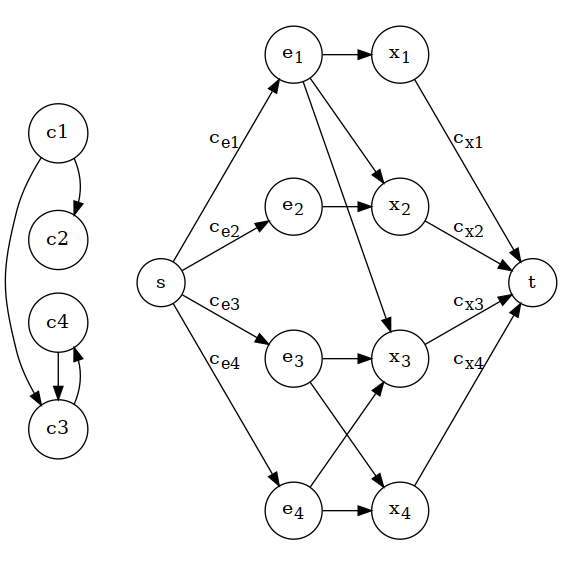
\includegraphics[scale=0.45]{txgraph1}
\end{figure}

\begin{lemma}
  Максимальный поток в графе $D$, построенному из $Tx$ и $G_c$ по
  вышеуказанному алгоритму равен $\sum_{i=1}^n{c_{en}}$
  $\Leftrightarrow$ покраска монет в $Tx$ удовлетворяет графу
  конвертации $G_c$.
\end{lemma}
\begin{proof}
  Пусть дано разбиение $H$ удовлетворяющее свойству \ref{eq:1}. В
  графе $D$ нулевой поток: $\forall uv \in D, \ f(u,v) = 0$. Для
  каждого цвета выхода $c_{out}$, его номинала $n_{out}$ и
  соответствующего $H_i = (n_{in}, c_{in})$ мы знаем, что $n_{out} =
  n_{in}$, а ребро $c_{in}c_{out} \in G_c$. Значит, в $D$ существует
  ребро между соответствующими вершинами долей. Примем $f(e_i,x_j) =
  n_{in}$ для соответствующих $e_i \sim c_{in}, \ x_j \sim x_j$, а
  также добавим $n_{in}$ к $f(s,e_i)$ и $f(x_j,t)$. Средние ребра
  имеют $c = \inf$ , а возможность насытить $se_i$ и $x_jt$ следует из
  свойств $H$ (разбиение эквивалентно $txIn$, значит для конкретного
  цвета мы не можем превысить суммы входов по этому цвету) и
  $txOut$. По окончании процедуры мы полностью заполним потоком каждое
  $x_jt$, поскольку мы итерировались по всем выходам транзакции, и
  каждое $se_i$, поскольку был перебран весь $H$. Таким образом, через
  граф был пропущен максимальный поток $f = \sum_{c \in txIn}{c}$.

  Обратное доказательство тривиально и проводится абсолютно
  аналогично. Для каждого ребра между долями $e_ix_j$ строится
  соответствующий $H_k$, объединение $H$ эквивалентно $txIn$ по
  построению.
\end{proof}

В общем случае $D$ содержит $O(mn)$ ребер из-за средней части графа,
построенной из $G_c$; количество вершин равно $m+n+2$. Поэтому среди
алгоритмов решения задачи о максимальном потоке, представленных в
\cite{goldberg1988new}, стоит отдать предпочтение тем, которые не
учитывают в асимптотике $E$: к примеру, \cite{malhotra1978v}
предлагает решение за $O(V^3)$, работающее для ациклических графов
(несложно проверить, что $D$ является ациклическим). На практике же
достаточно применить алгоритм Диница \cite{dinitz2006dinitz},
поскольку количество итераций алгоритма для практических задач обычно
невелико, а каждая итерация выполняется за $O(VE) = O(mn(m+n))$.

\subsection{Конкретная инстанциация и обратная совместимость}

Опишем множество $Col$. В реализации можно взять $Col =
\mathbb{B}^{32} \cong Int32$. Монеты цвета $basec \in Col$ считаются
базовыми монетами. Базовые монеты обратно совместимы с первоначальной
единственным типом монеты. Два других типа монет -- $ratec, \tau c \in
Colors$ будут использоваться для представления пользовательского
рейтинга в системе и очков времени соответственно. Последняя группа
монет -- монеты действия $actc_i$. Размер этого множества можно, для
простоты, взять дополнением $Colors$ за вычетом упомянутых ранее
тегов, то есть $N_a = |Colors|-3$, отсюда обозначим множество $actc =
\{actc_i\}_{i=1}^{N_a} \subset Colors$. В настоящей реализации
разумнее отвести на $actc$ меньшее пространство и уделить остаток
$Col$ на пользовательские нужды.

Используемый граф конвертации цветов $G_c$ будет иметь следующую
форму:
\begin{align*}
  E &= \{basec, ratec, \tau c\} \cup actc,\\
  V &= \{basec \rightarrow ratec
  , basec \rightarrow \tau c\} \cup
  \{\tau c \rightarrow actc_i\}_{i=1}^{N_a} \cup
  \{actc_i \rightarrow \tau c\}_{i=1}^{N_a}
\end{align*}

Таким образом, он включает в себя два односторонних правила
преобразования и одно двухстороннее для каждой пары $(\tau c, actc_i)$.

Приведем несколько замечаний о реализации. Предполагается, что
реальная стоимость одной монеты пренебрежима (единица монеты в
биткоине -- сатоши -- стоит $0.00001$ USD). В общем случае введем
функцию $roundMin : \mathbb{N} \rightarrow \mathbb{N}$, округляющую
значение интервала в минутах с нужной точностью. Тег в бинарном
(сериализованном) представлении монеты может быть опущен, и по
умолчанию равен $basec$.

Что касается гарантий стабильности протокола Ouroboros, предлагается
поддерживать только $basec$ во всех частях алгоритма, связанных с
размером сбережений:

\begin{enumerate}
\item SSC/выбор лидеров: к участию допускаются только участники с
  количеством монет $basec$ больше $sscThreshold$. Процедура выбора
  лидеров основывается на $basec$ балансах.
\item Система поощрений: поскольку разница между входами и выходами
  транзакции может быть только в монетах типа $basec$, все поощрения
  выплачиваются тоже в базовом цвете. Оплата увеличивает шансы
  эндорсеров и слот лидеров быть выбранными и не нарушает посылок
  доказательства о приближенном равновесии по Нэшу системы поощрений,
  описанной в \cite{ouroboros}.
\item Механизм делегации: запрещено делегировать средства другого
  любого цвета кроме $basec$, что не меняет схему.
\end{enumerate}

Легко видеть, что эта модификация не затрагивает гарантий базового
протокола, потому что изоморфна бесцветной схеме:

\begin{enumerate}
\item Не существует возможности получить $basec$ монеты из любого
  другого цвета.
\item Общая потеря $basec$ монет при конвертации не меняет поведения,
  потому что базовая реализация позволяет уничтожать монеты: отправляя
  средства на адреса с неизвестным секретным ключом или выставляя
  ненулевую разницу между входами и выходами транзакции (в случае
  отсутствующей реализации системы поощрений).
\end{enumerate}

\section{Система контрактов}

Контракт -- формализация способа взаимодействия пользователей как
множества обязательств и потребностей, а также соответствия
пользовательский действий в его рамках пользовательскому
рейтингу. Главная цель этой секции состоит в описании обязательств
таким образом, чтобы, имея данные о том, какие относящиеся к контракту
действия были выполнены (и в какой мере), пользователям можно было бы
проставить соответствующий рейтинг. Этот рейтинг должен коррелировать
с усилиями пользователей в отношении правил контракта и мотивировать
участников выполнять свои обязательства.

\subsection{Обязанности и потребности}

Представим условие контракта в виде набора обязанностей. Обязанность в
общем виде описывается следующими параметрами:

\begin{enumerate}
\item Тип деятельности $at \in actc$: любая активность, имеющая начало
  и конец. Например, парное программирование или какой-либо вид
  спорта.
\item Временн\'{о}е ограничение: $tr = (\tau_n, r_n)$, где $\tau_n$ --
  целевое количество времени в $period$, а $\tau_n \in N$ --
  минимальное необходимое количество транзакций. Некоторые типы
  деятельностей очевидным образом не входят в это описание из-за их
  случайной природы и невозможности автоматической проверки (например,
  условная деятельность ``прогулка в парке, если не идет дождь''). Тем
  не менее, ограничение по времени покрывает большую долю необходимых
  договоренностей.
\item Поставщики $supp$: пользователи, ответственные за то, чтобы
  обязательство было выполнено. В случае невыполнения требований,
  теряют свой рейтинг. Описываются множеством $\{U_0,
  U_1,\ldots,U_k\}$, что концептуально соответствует
  дизъюнктивной нормальной форме без отрицания: каждое $U_i$ это
  набор участников, допущенный к выполнению обязанности. Такое
  представление одновременно предоставляет необходимую гибкость и
  значительно упрощает валидацию при подсчете рейтинга.
\item Получатель $rec \in U_c \sqcup \{u_{\varnothing}\}$: тот, кто
  определяет необходимость в совместном времяпровождении. Получатель
  -- пользователь, вместе с которым эта активность должна
  происходить. Групповые деятельности, в которых получателем является
  каждый участник, описываются множеством обязанностей (по одной на
  удовлетворения потребностей каждого). Для активностей без явного
  получателя это поле имеет значение $u_{\varnothing}$. Пример: Алиса
  или Боб обязаны производить уборку помещения в течение 4 часов
  еженедельно -- в этой активности нет явного получателя, а поставщики
  $\{\{A\}, \{B\}\}$. Также добавим ограничение $supp \cap rec =
  \varnothing$, исключающее получателя из множества поставщиков..
\end{enumerate}

Таким образом $rs \in Resp_c$, где $Resp_c$ -- множество обязанностей
в контракте $c$, имеет следующую форму: $rs = (supp, rec, at, tr)$. Мы
будем прибегать к нотации $supp \rightarrow rec$ для краткого описания
только двух полей. Функция $Users(R)$ возвращает $\{ u \mid supp(rs)
\sqcup rec(rs), \ rs \in R \}$. Такая формализация обязанности $rs$
является достаточно широким, чтобы покрывать большинство необходимых
ситуаций и в то же время простым, что позволяет автоматизировать
процесс выставления рейтинга.

Частым случаем является набор ответственностей $R = \{rs_i\}_{i=0}^k$,
имеющих одно множество $U_R = Users(rs_i), \ \forall i $, причем
$\{supp(rs_i)\}$ покрывает все сочетания на $U_r$ размера $k-1$. Такой
набор характеризует договоренность группы лиц заниматься деятельностью
строго в группе. Пусть $R \subset Resp_c$. Построим ориентированный
граф $G$, приняв $E = U_r$ и $V = \bigcup_{rc \in Resp_c}{\{v_jr \mid
  rc = \{v_1\ldots v_{s(j)}\} \rightarrow r\}}$. Преобразуем $G$ в
$F$: оставим вершины, но добавим $vr \in G$ в $F$ только если $vt \in
G \wedge tv \in G$. Заметим, что каждый $R$ подходящий под условия
соответствует клике в $F$ на вершинах $U_R$. Это замечание может быть
применено для эффективного кодирования $Resp_c$.

\subsection{Скрипт контракта}

Эта секция описывает схему интеграции контракта в скрипт
криптовалюты. Скрипт-адрес представляет из себя аккаунт, который
поддерживает единственную операцию снятия с себя средств --
продление. Продление контракта представляет собой транзакцию, которая
распределяет рейтинг по выделенным дополнительным адресам,
ассоциированным с этим скриптом. Чтобы инициировать контракт,
необходимо создать скрипт и перевести $basec$ монеты на его счет.

Сам код скрипта делится на две части -- встроенный код и
конфигурацию. Конфигурация -- это темплейтные поля, которые
заполняются пользователем. Она содержит в себе следующие параметры:

\begin{enumerate}
\item Период контракта $period$. Поскольку Ouroboros имеет встроенную
  поддержку слоттинга с фиксированной длиной слота, то пользователь
  может указать период в слотах, а скрипт может оперировать этим
  понятием с хорошей точностью (доставать все транзакции за выделенный
  период времени).
\item Метка старта контракта $start$. Для того, чтобы контракт мог
  выделить последний период, ему необходимо знать слот, в котором
  появилась последняя транзакция продления (это можно сделать с
  помощью встроенных в скриптовый язык функций). Но до первого
  продления эта информация не существует. Метка старта представляет из
  себя индекс слота и используется ровно в этом случае.
\item Множество участников контракта $U_c$.
\item Множество обязательств $Resp$, построенное на $U_c$.
\item Расширенный публичный HD ключ $CPke$, который будет в дальнейшем
  использован для построения адресов активностей.
\end{enumerate}

Отдельно необходимо выделить, что имея темплейт скрипта, мы всегда
можем проверить, подходит ли под него конкретная
инстанциация\footnote{Эта возможность используется в биткоине --
  скрипты, не подходящие под фиксированный список темплейтов, не
  распространяются клиентами
  \url{https://github.com/bitcoin/bitcoin/blob/master/src/script/standard.cpp}}. Это
дает возможность выявлять и игнорировать модифицированные скрипты.

Таким образом, внутреннее состояние контракта характеризуется, в
первую очередь, его последним периодом $c\Delta = [siLast \ldots
siLast+period]$, где $siLast$ -- функция, возвращающая слот
последней транзакции продления или $start$, если транзакции
отсутствуют. Для ее реализации необходимо добавить в plutus поддержку
встроенного примитива $searchTx$, который с помощью ресурсов узла сети
произведет поиск по транзакциям, соответствующим предикату. В случае
$siLast$ необходимо найти последнюю транзакцию перевода средств с
публичного адреса скрипта. После того, как $c\Delta$ определен, скрипт
производит поиск всех трекинг-транзакций в этом периоде, считает
рейтинг для каждого пользователя и удостоверяется, что распределение
рейтинга в транзакции соответствует подсчитанному.

\subsection{Схема транзакций}

Транзакция активности несет в себе информацию об одном виде активности
и том, сколько каждый ее участник потратил на нее времени. Обозначим
за $U_{tx} = \{u_i\}_{i=1}^N$ множество пользователей, участвующих в
деятельности типа $at = actc_k$ для некоторого $k$ в рамках контракта
$c$. $T_i = (\tau S_i, \Delta_i)$ -- временной промежуток (пара из
начала и длительности, в POSIX миллисекундах и минутах
соответственно), соответствующий реальной активности пользователя
$u_i$, $T = \{T_i\}_{i=1}^N$ Тогда определим пред-транзакцию как
$ActionTxPre = (U_{tx}, T, at)$. Эта модель удовлетворяет требованиям,
предъявляемым контрактом, но несет в себе избыточную информацию о
реальном времени. Необходимо знать две вещи: когда произошла
транзакция (эта информация выводится из слота блока, в который
транзакция попадет) и сколько времени пользователи потратили на
каждого другого участника транзакции в ее же рамках. Заметим, что
последнее замечание критично ввиду потенциально нетривиального
пересечения отрезков из множества $T$.

Чтобы построить реальную транзакцию активности $ActionTx$, нам
потребуется превратить $ActionTxPre$ в два списка -- входы и выходы
транзакции (списки $(address,amount,color)$). Пусть $Pk_i$ --
публичный ключ $u_i$. Введем функцию $CActOut(C, U_i) : Pk$, которая
по контракту и непустому подмножеству пользователей $U_i \subset U$
возвращает публичный ключ. $CActOut$ инъективна и имеет конечное множество
значений размера $2^N = \sum_{i=1}^N{\binom{N}{i}}$. Эта функция
используется для того, чтобы ассоциировать контракт с адресами
активности, на которых будут накапливаться $actc_i$.

Пусть $E_s = \{ev_i\}_{i=1}^k$ есть множество всех событий из
интервалов в $T$, где событием является начало или конец промежутка --
$T_{st}(T_i) = \tau S_i$ или $T_{fin}(T_i) = \tau S_i +
\Delta_i$. Легко видеть, что для каждого выделенного интервала из
$\{[ev_i, ev_{i+1}]\}_{i=1}^{k-1}$ есть ровно одно активное
подмножество пользователей $U_i \subset U$. Для каждого $u_i$ и его
$T_i$ поделим $\Delta_i$ на множество интервалов $\{\Delta_{i,j}\}$,
разбивая в соответствии с $E_s$: $\sum_{j}{\Delta_{i,j}} = Delta_i$,
$Delta_{i,1} = [ev_h, ev_{h+1}]$ для некоторого $h$, $Delta_{i,j} =
[Ev_{h+j},Ev_{h+j+1}]$. Построим множество соответствия $Compl_i$: по
каждому интервалу $\Delta_{i,j}$ получим $ActPk_{i,j} = CActOut(C,
U_j)$ и объединим все $\{(\Delta_{i,j}, ActPk_{i,j})\}$, имеющие
одинаковый публичный ключ, суммируя по $\Delta_{i,j}$, чтобы избежать
дубликатов. Обозначим это множество пар за $Compl_i$ и примем его
размером $M_i$. Таким образом, $Compl_i$ содержит информацию о том,
сколько времени $u_i$ взаимодействовал с каждым другим участником
транзакции.

Эта процедура проводится для каждого пользователя. Далее множество
$\{Compl_i\}_{i=1}^N$ может быть напрямую преобразовано в
транзакцию. $u_i$ определяет $(\tilde{\Delta}_i, \tau c)$ как вход
своей подтранзакции, где $\tilde{\Delta}_i =
\sum_{s=1}^{M_i}(\Delta_{i,s})$, и для каждого $(\Delta_{i,j},
ActPk_{i,j}) \in Compl_i$ выставляет выход в соответствующее
$\Delta_{i,j}$ количество монет, адрес $ActP_{i,j}$ и цвет монеты
$at$. Все подтранзакции объединяются в одну, конкатенируя входы и
выходы соответственно. В конечном счете, $ActionTx$ имеет $(Pk_i,
\tilde{\Delta}_i, \tau c)$ на входах для каждого участника, а на
выходах $(ActP_{i,j}, \Delta_{i,j}, at)$. Мнемонически, участник
разбивает свои временн\'{ы}е ресурсы $\tau c$ в размере потраченного
времени на ресурсы действия $at$.

Валидность транзакции относительно балансов очевидна по построению,
так как сумма входных монет для каждой подтранзакции определяется
через сумму выходов и выполняется правило перекрашивания $\tau c
\rightarrow at$. После преобразования, $ActionTx$ не содержит
излишней информации о метках времени.

\section{Функционал адресов активностей}

Инстанциируем функцию $CActOut(C, U)$, использованную ранее для вывода
множества публичных ключей из контракта и подмножества его
пользователей. Одним из требований к ней является возможность
генерировать парные (к публичным) секретные ключи. Это поможет
переиспользовать $actc_i$, конвертируя их обратно в $\tau c$. Также,
хотелось бы минимизировать информацию, идентифицирующую эту функцию в
скрипте, поскольку валидаторы хранятся в блокчейне явно. Наивный
подход хранения списка публичных адресов является избыточным по
памяти. Решение, предлагаемое в этой главе, заключается в
использовании расширенных HD ключей.

Выделим среди пользователей контракта одного (мастера) и предположим,
что он владеет расширенным секретным ключом $CSke$. Публичная
компонента этого ключа $CPke$ находится в конфигурации
валидатора. Определим функцию $CactOut(C,U)$ следующим образом:

\begin{enumerate}
\item Занумеруем все сочетания на $U_c$ с помощью $userEnum : 2^{U_c}
  \rightarrow \mathbb{N} / 2^N$. $userEnum$ может быть определена
  тривиально. Представим $U_i$ с помощью целого $i \in \mathbb{N}$, а
  каждое $U_j \subset U_c$ в виде отсортированного списка его
  элементов, представленных натуральными числами. Тогда порядок на
  $\{U_j\}$ может быть определен лексикографически.
\item $CActOut(C,U_j) = CPke/userEnum(U_j)$. Напомним, что запись
  $Pke/i$ означает выведенный из $Pke$ дочерний публичный ключ номер
  $i$ .
\end{enumerate}

Не смотря на то, что мастер единолично владеет критическим знанием о
секретном ключе контракта, это не нарушает существующих гарантий
безопасности протокола. Во-первых, мастер не имеет возможности
повлиять на распределение рейтинга в контракте, поскольку оно
гарантируется самим скриптом. Более того, наличие реальных средств на
рейтинговых адресах тоже не является необходимым условием для
успешного распределения рейтинга -- скрипт ориентируется на сами
транзакции, а не на существующие непотраченные выходы транзакций (даже
если мастер снимет все средства, контракт будет успешно
выполнен). Во-вторых, имеет место допущение про то, что цена $actc_i$
пренебрежимо мала, поэтому мастер не имеет мотивации манипулировать
этими средствами. В-третьих, любой участник контракта все еще может
провести транзакцию обновления, без перевода средств с адресов
активности.

Альтернативная модификация схемы, устраняющая централизованное
владение $CSke$, предполагает неявное создание $2^N$ скрипт-адресов в
$CactOut$, средства с которых может списывать любой участник
контракта. Минус схемы в её более высокой сложности описания и
потенциальном увеличении размера блокчейна количеством валидаторов
(доказательства транзакций хранятся в блоках). Поэтому схема с
использованием HD ключей является более оптимальной для описания
протокола.

\section{Функция распределения рейтинга}

Функция распределения рейтинга определяется как:
\[RateAssign : Resp \times Txs \times U_c \rightarrow \mathbb{N}\]
где $Txs = {ActionTx_i}_{i=1}^M$ -- набор транзакций из последнего
периода контракта, а возвращаемое значение -- рейтинг.

Рейтинг определяет соответствие действий пользователя его
обязанностям. Его реальная область значений для $u_i$ принимается
равной $[0,\theta_i]$, где $\theta_i < period$. $\theta_i$ представляет
собой количество времени во всех контрактах, за которые $u_i$
ответственен. Рейтинг, коррелирующий с длительностью обязанностей
контракта, выбран по причине высокой репрезентативности и наглядности,
а также независим от субъективных оценок пользователей.

Для каждой $ActionTx_i$ определим $tx_i : 2^{U_c} \rightarrow N$,
возвращающая по $U \subset U_c$ количество монет на первом выходе
$ActionTx_i$, имеющем адрес $CActOut(U)$. Пусть $tracks(tx_i) = \{
(U,v) \mid v = Tx_i(U) \wedge v \neq 0 \}$. Рассмотрим единичную обязанность $rs =
supp \rightarrow rec \in Resp$, пусть $S = \bigcup_{i=1}^{k}{supp_i}$.

Определим важность пользователя $\psi_{rs}(u_i) = \phi_{U_i}(v)$, где
$v(X) = |2^X \cap supp|$ -- характеристическая функция, а $\phi$ --
вектор Шепли \cite{shapley} \cite{petrosyan}. $v(U_i)$ показывает,
сколькими способами коалиция $U_i$ могла бы подойти под требования
$supp$. Поскольку $sum_i{\phi_{U_i}(v)} = v(S) = 1$, то вектор
$\{\psi_{rs}(u_i)\}_i$ определяет веса важности для
участников. Наглядным примером использования является $supp =
\{\{1\},\{2\},\{1,3\}\})$ с выходным вектором $\psi = (\frac{1}{3},
\frac{1}{2}, \frac{1}{6})$, который иллюстрирует низкую важность
пользователя $3$, поскольку он может участвовать в $rs$ только вместе
с $1$.

Определим функцию временн\'{о}й потери. Пусть $Txs_{rs}$ есть
множество транзакций, относящихся к $rs$ (имеют цвет $ac_{rs}$,
пользователи только из $Users(rs)$). Напомним, что $\tau_n$ есть
целевое время выполнения $rs$, $r_n$ -- количественное (в
транзакциях). $\tau_r = \sum_i{\tau_{r,i}},\ \tau_{r,i} = \{r | (U,r)
= tracks(tx_j),\ rec \in U, \ tx_j \in Txs_{rs}\}$ есть реальное время,
  потраченное в рамках $rs$ с пользователем $rec$. По аналогии $r_r$
  -- количество проведенных транзакций. В случае $rec =
  u_{\varnothing}$ условие $rec \in U$ опускается.

\begin{align*}
l =
\begin{cases}
  \tau_{\delta} = \tau_n - \tau_s, & \text{если } \tau_n = 0 \\
  \theta + \max{(0, \tau_r - \theta)}, \ \text{где} \ \theta = \frac{\tau_n}{r_n}r_r, & \text{иначе}
\end{cases}
\end{align*}

Таким образом, видно, что $l \leq \tau_n$, причем $l = \tau_n$
показывает полную невыполненность обязательства. Значение потери $l$
пользователи $u \in supp$ распределяют в качестве штрафа.

Учтем также время, потраченное пользователями на удовлетворение
$\tau_r$. Определим количество времени, проведенных $u_i$ вместе с
$rec$ в рамках этого обязательства и $Tx_{rc}$

\begin{align*}
  &com_{i,j} = \{r \mid (U,r) = tracks(tx_j),\ \{u_i, rec\} \subset U, \ tx_j \in Txs_{rs}\} \\
  &com(u_i) = min{(\sum_j{com_{i,j}}, \ \psi(u_i) \tau_r)}
\end{align*}

Тут $com(u_i)$ -- доля времени $u_i$, учитывающаяся в расчете рейтинга. Следующий блок функций рассчитывает сам рейтинг:

\begin{align*}
  &d_{rs}(u_i) = \psi_{rs}(u_i)\tau_{n,rs} \\
  &p_{rs}(u_i) = \frac{d_{rs}(u_i) - com_{rs}(u_i)}{d_{rs}(u_i)} l_{rs} \psi_{rs}(u_i) \\
  &p_t(u_i) = \sum_{rs \in Resp}{p_{rs}}, \ \ \ p_m(u_i) = \sum_{rs \in Resp}{d_{rs}(u_i)} \\
  &r_f(u_i) = p_m(u_i) - p_t(u_i)
\end{align*}

$d_{rs}\tau_{n,rs}$ это количество времени, которое $u_i$
ответственен в $rs$. $p_t$ -- общий (total) штраф $u_i$ по всем
$rs$. $p_m$ это максимальное количество времени, которое $u_i$ должен
уделять на $rs$ исходя из $\psi_{rc}(u_i)$ и $\tau_n$ для каждого $rs
\in Resp$. $r_f(u_i)$ это финальный рейтинг $u_i$. $RateAsign(u_i) =
r_f(u_i)$.

\begin{lemma}
Функционал $r_f$ имеет следующие свойства:
\begin{enumerate}
\item Заполнение: $\forall rs \mid u_i \in supp(rs) . \ l_{rs} = 0
  \Leftrightarrow r_f(u_i) = p_m(u_i)$. Пользователь получает максимальный
  рейтинг только если удовлетворяет всем своим обязанностям.
\item Аксиома болвана: $\forall rs \mid u_i \in supp(rs) . \ l_{rs} = \tau_{n,rs}
   \wedge com_{rs}(ui) = 0 \Rightarrow r_f(u_i) = 0$. Пользователь
  получает нулевой рейтинг, если для каждой его обязанности она не
  была выполнена и его $com(u_i) = 0$.
\item Монотонность: для выделенного $rs$ при $com_{rs}(u_i) \leq
  com_{rs}(u_j)$ и $\psi_{rs}(u_i) = \psi_{rs}(u_j)$ верно
  $p_{rs}(u_j) - p_{rs}(u_i) \ge 0$. При равной важности пользователь
  больший штраф получает тот, чей $com$ меньше.
\end{enumerate}
\end{lemma}
\begin{proof}
Ограничение суммы $com_{i,j}$ значением $\psi(u_i) \tau_r$ имеет
следующее свойство: $l \ge 0 \Rightarrow com(u_i) \le d(u_i)$, причем
равенство достигается только одновременно. Также отметим, что $u_i
\notin supp(rs) \Rightarrow \psi_{rs}(u_i) = 0$, а значит $d_{rs}(u_i)
= 0$. Отсюда обозначим $Resp(u_i) = \{rs \in Resp \mid u_i \in
supp(rs) \}$ -- очевидно, что в сумме $r_f$ элементы по $rs \notin
Resp(u_i)$ будут вносить нулевой вклад.

Покажем выполнение свойства (1). Пусть $l_{rs} = 0$ для всех
рассматриваемых контрактов.
\begin{align*}
  r_f &= \sum_{rs \in Resp(u_i)}{d_{rs}(u_i)  -  \frac{d_{rs}(u_i) - com_{rs}(u_i)}{d_{rs}(u_i)} l_{rs} \psi_{rs}(u_i)} \\
      &= \sum_{rs \in Resp(u_i)}{d_{rs}(u_i)} = p_m(u_i)
\end{align*}

Множитель $\frac{d_{rs}(u_i) - com_{rs}(u_i)}{d_{rs}(u_i)}$ строго
положителен при $\psi_{rs}(u_i) \ge 0$ из-за вышеописанных свойств
$com_{rs}(u_i)$. Аналогично выполняется второе свойство. Пусть $l_{rs}
= \tau_{rs,n}$, и $u_i$ имеет $com_{rs} = 0 , \ rs \in Resp(u_i)$.
\begin{align*}
  r_f &= \sum_{rs \in Resp(u_i)}{d_{rs}(u_i)  -  \frac{d_{rs}(u_i) - com_{rs}(u_i)}{d_{rs}(u_i)} l_{rs} \psi_{rs}(u_i)} \\
      &= \sum_{rs \in Resp(u_i)}{d_{rs}(u_i)(1  -  \frac{d_{rs}(u_i)}{d_{rs}(u_i)})} = 0
\end{align*}

Третье свойство также показывается прямолинейно. Если $\psi(u_i) =
\psi(u_j) = \psi$, то и $d(u_i) = \tau_n \psi = d(u_j) = d$. Отсюда:
\begin{align*}
p_{rs}(u_j) - p_{rs}(u_i) = l \psi \frac{d - com(u_j) - d + com(u_i)}{d} = l \frac{com(u_i) - com(u_j)}{\tau_n} \ge 0
\end{align*}

\end{proof}

Также очевидно, что участие пользователя в обязанности, которая не
была выполнена полностью, влечет снижение $r_f(u_i)$, а также $\forall
rs \in Resp . \ r_f(u_i) \sim com_{rs}(u_i)$.

\section{Транзакция продления и поток активов}

Единственный способ, с помощью которого с контракта можно переводить
средства, есть транзакция продления контракта. Она состоит из двух
частей:

\begin{enumerate}
\item Плата за продление в $basec$. Эти монеты переходят на
  специальные рейтинговые адреса ${CRewPk_i}_{i=1}^N$. Также, эта часть
  транзакции должна быть использована для оплаты самой транзакции.
\item Опционально, объем монет типа $actc$, которые участвовали в
  трекинговых транзакциях, и накапливались на адресах
  $CActOut(C,U_i) \mid U_i \subset U$. Эти средства могут быть
  переиспользованы. Соответствующий выход может иметь любой адрес и
  тип выходных средств $\tau c$. Предполагается, что мастер контракта
  переводит эти средства себе, либо другим участникам для дальнейшего
  оборота.
\end{enumerate}

Рейтинговые адреса формируются из публичных ключей, которые выводятся
из контракта и публичного ключа пользователя. Они не имеют
соответствующих секретных ключей намеренно, что гарантирует
невозможность снять $ratec$ со счета и скрыть статистику. В качестве
реализации можно взять $CRewPk_i = Blake2b_{512}(CPk || UPk_i)$, где
$Blake2b_{512}$ это хэш-функция из семейства
blake2\footnote{\url{https://blake2.net/blake2.pdf}} с размером
хэш-пространства $2^{512}$ (чтобы совпадать со схемой расширенных HD
ключей).

Опишем полную схему потока активов.

\begin{enumerate}
\item Группа пользователей создает скрипт, добавляя в темплейтные поля
  конфигурационные параметры. Один пользователь назначается мастером:
  он генерирует $CSke$ и добавляет $CPke$ в конфигурацию. Любой
  участник переводит $basec$ монеты на счет $CPk$, чтобы инициировать
  контракт.
\item Первым периодом контракта является $[start,
  start+period]$. Пользователи самостоятельно меняют $basec$ на $\tau
  c$ (или получают $\tau c$ любым другим способом) и отмечают свои
  действия в рамках периода контракта с помощью транзакций активности.
\item Начиная со слота $start + period + 1$ мастер может продлить
  контракт. Он создает транзакцию продления, собирая информацию о
  действиях за последний период, выставляет соответствующую плату за
  транзакцию, добавляет подписи для $CActOut$ ключей (с помощью
  $CSke$) и отправляет транзакцию в сеть.
\item Узел сети, проверяющий транзакцию, произведет проверку балансов
  и расчет платы транзакции. За этим следуют проверки валидности всех
  потраченных входов транзакции. $CActOut$ входы будут проверены с
  помощью приложенных мастером подписей, затем узел запустит валидатор
  (с пустым ридимером).
\item Валидатор имеет доступ к блочейну и текущей обрабатываемой
  транзакции. Он производит следующие проверки:
  \begin{enumerate}
  \item Выводит последний период (с помощью $siLast$ и $period$) и
    проверяет, что текущий период больше правой границы интервала.
  \item Транзакция продления подходит под общий темплейт: два типа
    входов ($CPk$ и $CActOut_i$), два типа выходов ($CRewPk_i$ адреса,
    типа выхода $ratec$; $\tau c$ тип выхода на всем остальном).
  \item Входы соответствующие адресам активностей, в точности
    совпадают со всем множеством входов, использованных в последний
    период. Валидатор имеет возможность производить поиск по
    транзакциям (с помощью реализованного узлом примитива), поэтому
    проверка сводится к сопоставлению множеств.
  \item Распределение наград на выходе транзакций соответствует
    подсчитанному валидатором (с помощью $RateAssign$).
  \end{enumerate}
\item Транзакция продления попадает в блокчейн, распределяя очки
  рейтинга. Транзакция продления начинает новый период. Пользователи
  могут продолжить сценарий со второго пункта.
\end{enumerate}

\section{Формирование транзакций}

Для того, чтобы транзакции активности могли попасть в блокчейн, они
должны быть подписаны каждым участником. Стандартные подходы для сбора
подписей в мультипользовательских транзакциях в основном делятся на
ручные (передача подписи текстом или с помощью QR кода, например в
клиенте
electrum \footnote{\url{http://docs.electrum.org/en/latest/multisig.html}})
и на автоматические, с использованием централизованного пула
подписей\footnote{Централизованный сбор подписей в кошельке coinkite:
  \url{http://blog.coinkite.com/post/102291566521/bitcoin-multisig}}. Подход,
необходимый для формирования $PreActionTx$ и последующего сбора
подписей для $ActionTx$, более комплексный. Разделим функционал на две
части: логика и транспорт. Под логическим слоем подразумевается API
приложения. Транспорт -- физическая реализация. Мы рассмотрим
возможные решения транспорта, связанные с централизованными серверами
и децентрализованной сетью.

\subsection{Логический слой}

Главная идея этой части функционала -- предоставить пользователям
интерфейс для создания пре-транзакции и автоматизировать сбор подписи
после. Предложенный API хранит пре-транзакции, идентифицируемые
суррогатным ключом $preTxId$ и сконвертированные транзакции по их
хэшу $txHash$. Логика API со стороны транспорта предоставляет
следующие методы:

\begin{enumerate}
\item $StartActivity(IPk, \{UPk_i\}, actc_k, CInfo, desc) : txid$. Этот
  вызов инициирует пустую пре-транзакцию. Инициатор прикладывает свой
  публичный ключ, публичные ключи других участников и подписывает эту
  информацию своим ключом. Также он прикладывает информацию о типе
  активности и информацию о контракте (которая в общем случае
  неизвестна узла). Вызов возвращает идентификатор пре-транзакции.
\item $ChangePermissions(\{UPk_i\}, cmd) : \{UPk_i\}, cmd \in
  \{grant,revoke\}$. Вызов изменяет настройки доступа к
  транзакции. Мастер может приглашать или удалять приглашенных
  участников. Возвращаемое значение -- множество участников, для
  которых удалось применить данную операцию.
\item $SearchTx(args) : List(match), match \in \{(preTxId,extra),
  (tx,preWitness)\}$ производит поиск по пре-транзакциям и транзакциям,
  удовлетворяющим требованиям заданным в $args$. Предполагается
  поддержка поиска по публичному ключу приглашенных участников (или
  мастера), также по идентификаторам. Возвращает:
  \begin{enumerate}
  \item Пре-транзакции, подходящие под требования, с дополнительной
    информацией в случае, если участник приглашен в пре-транзакцию.
  \item Транзакцию $tx$ с возможно неполным списком подписей $witness$.
  \end{enumerate}
\item $PreTxStart(txid, UPk_i, time) : Bool$ отмечает начало
  временн\'{о}го интервала для пользователя. Возвращает значение,
  свидетельствующее об успехе операции (далее аналогично).
\item $PreTxExit(txid, UPk_i, time) : Bool$ завершает временн\'{о}й
  интервал для указанного пользователя.
\item $UploadRawTransaction(tx, \sigma) : Bool$ загружает в транспорт
  сырую транзакцию с подписью одного из участников.
\item $UploadSignature(UPk_i, \sigma, txHash) : Bool$ загружает
  подпись участника $\sigma$ в соответствующий транзакции
  $prewitness$.
\end{enumerate}

Полностью законченные пре-транзакции автоматически конвертируются в
транзакции без подписей, последние могут быть индексированы с помощью
$SearchTx$. Любой участник отправляет готовую транзакцию с подписями в
сеть.

Этот слой логики также удаляет всю информацию, находящуюся в
транспортном слое слишком долго, снижая нагрузку на транспорт и
ограничивая время одной пре-транзакции. Для того, чтобы избежать
перегрузки сервиса, транспорт может быть либо приватным, либо быть
синхронизированным с блокчейном и допускать к использованию только
участников, имеющих достаточно средств (подход, применяемый в
нескольких компонентах Cardano SL).

В случае, если между участниками возникает спорная ситуация о том,
стоит ли подписывать транзакцию, по её разрешении любой может
загрузить пре-транзакцию локально, изменить, сконвертировать в
транзакцию и предложить ее на подпись с помощью
$UploadRawTransaction$.

\subsection{Транспортный слой}

Реализация транспорта может быть централизованной или
распределенной. Требования, предъявляемые к архитектурному решению:
\begin{enumerate}
\item Отказоустойчивость: сервис не должен терять данные в случае
  сбоя. Решается тривиально в централизованных сервисах (большинство
  ДБ поддерживают durability) и авторизованных децентрализованных (та
  же схема).
\item Политика хранения данных: физические ресурсы сервиса
  ограничены. Решением может быть вышеупомянутое удаление данных по
  таймауту, введение авторизации пользователей и лимита по памяти на
  пользователя (например, по публичному ключу пользователя $U_i$ в
  Cardano SL, где разрешенное количество пропорционально счету
  пользователя).
\end{enumerate}

Реализация централизованного сервера прямолинейна, но имеет очевидные
недостатки в виде необходимости доверять серверу (в случае, если он не
принадлежит участникам). С другой стороны, наивное распределенное
решение с помощью DHT (которое можно было бы реализовать поверх
существующей p2p сети) подвержено sybil атаке
\cite{dinger2006defending}. Сценарий атаки заключается в том, что при
большом количестве вредоносных узлов в сети нарушаются гарантии
роутинга и репликации данных в общем. Кроме общих решений описанных в
\cite{dinger2006defending}, и, в частности, применимых к Kademlia DHT
\cite{maymounkov2002kademlia} (которая используется для поиска пиров в
Cardano SL), описанных в \cite{wang2008attacking}, можно предоставить
простое решение, использующее интеграцию с Ouroboros.

Среди основных посылок, Ouroboros предполагает что ни один участник
сети не имеет больше половины всех средств в сети. Исходя из этого,
предлагается модифицировать Kademlia DHT, добавив два дополнительных условия:
\begin{enumerate}
\item Все вызовы авторизованы публичными ключами узлов, то есть имеют
  соответствующие подписи. Вызовы с неверными подписями
  игнорируются. При добавлении нового узла с ключом $Pk_i$ в k-бакет
  рассматриваемый узел проверяет условие $balance(Pk_i) >
  kadThreshold$ и производит добавление только в случае
  успеха. Другими словами, узлы в которой могут участвовать только
  узлы сети, имеющие количество средств выше заданного порога.
\item В начале каждой эпохи узел сети удаляет из каждого k-бакета все
  узлы, количество средств которых упало ниже $kadThreshold$.
\item $kadThreshold$ выбирается в зависимости от реального
  распределения средств в системе.
\end{enumerate}

\section{Модель взаимодействия, атаки и улучшения}

В предыдущих секциях было описано само решение для поддержки
функциональности тайм-трекинга. Эта секция уделяет внимание глобальным
и локальным свойствам рейтинга, а также возможным атакам, и гарантиям
контрактной системы, а также предлагает потенциальные улучшения схемы.

\subsection{Контракт и доверие}

По умолчанию предполагается, что система доверия внутри контракта
полная -- система предназначена для оптимизации активностей внутри
контракта, и каждый пользователь доверяет всем другим
участникам. Мультипользовательские транзакции имеют подписи всех
участников, поэтому они явно подтверждаются соответствующим набором
пользователей. Но система также допускает единичные обязанности вида
$u \rightarrow u_{\varnothing}$, транзакции которых подтверждаются
только одной подписью. Для того, чтобы элиминировать возможные
проблемы с доверием, предлагается следующее решение, основанное на
рецензентах транзакции.

Допустим, что в модели контракта есть набор обязанностей $R$,
выполняемый пользователями из $U_R$, и пользователь $u_m$, который
требует подтверждения всякой транзакции, удовлетворяющей $rs \in
R$. Введем в контракт множество пользователей $U_r$ (reviewers,
рецензенты). Добавим в обязанность $rs \in R$ поле $rv \subset 2^{U_r}$ --
множество пользователей, которые должны дополнительно подтверждать
транзакции, относящиеся к $rs$. Перед подтверждением тайм-трекинг
транзакции $tx$, она валидируется любым множеством рецензентов $rv_i
\in rv$ путем добавления входов транзакции, подписанного каждым $r \in
rv_i$. Соответствующий выход может также принадлежать $r$ (ему
достаточно отправить деньги самому себе в рамках $tx$). При подсчете
рейтинга транзакции, не имеющие подписи рецензентов, не будут входить
в целевое рассматриваемое множество. Таким образом $u_m$ может
форсировать дополнительную проверку транзакций необходимого
подмножества пользователей $U_R$.

Тривиальным примером является обязанность $rs$, выполняемая одним
пользователем типа $u \rightarrow u_{\varnothing}$. Остальные
пользователи контракта $U_R$ могут договориться, что каждая единичная
транзакция удовлетворяющая $rs$ должна иметь множество рецензентов
$\{\{u\} \mid u \in U_R\}$, то есть должна быть подтверждена любым
другим участником контракта.

\subsection{Особенности области применения}

Предложенная система, как и любое тайм-трекинг решение, разумно
распределяет рейтинг только при следующих условиях:
\begin{itemize}
  \item Пользователи ставят цель измерять {\it время},
    пропорциональное усилию, а не {\it результат работы}. Это
    предположение используется на любой длительной должности с
    фиксированной оплатой. Следствием является то, что любая
    активность имеет константную производительность.
  \item Долгосрочность: контракт заключается с расчетом не
    неограниченный срок. В случае, если целью контракта является
    получение некоторого блага (например, активность -- работа над
    проектом, который нужно сдать в срок), это вступает в противоречие
    с первым пунктом: заказчик проекта может предпочесть измерять не
    время работы, а реальную рабочую продуктивность пользователей. Эта
    возможность не поддерживается системой и не относится к
    тайм-трекингу.
\end{itemize}

\subsection{Рейтинг}

Исходя из текущей локальной модели доверия внутри контракта, выделим
некоторые свойства рейтинга.

Во-первых, можно установить лишь локальную правдоподобность
рейтинга. Поскольку реальное соответствие действий обязательствам
невозможно проверить глобально в отсутствии централизованного
источника доверия, любое закрытое множество пользователей может
создать контракт и максимально удовлетворять всем его
обязанностям. Предотвратить такое поведение в принципе не
представляется возможным: единственное отличие нечестных контрактов
заключается в несоответствие реальности данным о тайм-трекинге,
проверку чего невозможно автоматизировать.

Тем не менее, пользователь может провести аудит своих честных
контрактов, подтверждая их с помощью сторонних средств: живых отзывов
других пользователей, наличия в контракте доверенных участников в
качестве рецензентов и т.д. Также возможно применять различные методы
для кластеризации и автоматического нахождения нечестных контрактов и
помечать их подозрительными в приложении для проведения аудитов.

Во-вторых, сами монеты рейтинга $ratec$ могут быть получены любым
пользователем с помощью конвертации из $basec$. Но, как было уже
упомянуто в описании транзакции, любой участник сети может проверить,
подходит ли контракт под корректный темплейт. Имея эту возможность,
приложение может фильтровать учитывать только те $ratec$, которые были
отправлены со счета контракта, проходящего проверку, тем самым решая
поставленную проблему.

\subsection{Денежные штрафы}

Имея прямую интеграцию с криптовалютой, очевидной идеей является
интеграция реальных денежных средств в систему штрафов
контракта. Предложим две реализации этой идеи:

\begin{enumerate}
  \item Штраф, пропорциональный $p_n$ в расчете штрафа по
    $ratec$. Выставим ограничение на выполнение транзакции продления:
    дополнительным условием будет являться наличие на счету контракта
    залога в размере $\sum_{u_i \in U}{\alpha_i p_m(u_i)}$, где $U$ --
    множество пользователей контракта, а $\alpha$ -- вектор весов
    штрафа для каждого пользователя. Добавим возможность для каждого
    иного пользователя $u_j$ в любой момент после выпуска транзакции
    продления снять со счета контракта свою долю штрафа от $u_i$, где
    значение денежного штрафа есть $\sum{\alpha_i p_{rs}(u_i)}$ по
    всем $rs$, в которых $u_j$ выступает получателем. Транзакции и
    рейтинги рассчитываются за последний продленный период. Нетрудно
    показать, что залога хватит на максимальную общую сумму штрафов.
  \item Штраф за позднее продление. Выставим фиксированный штраф за
    несвоевременное (позже чем $siLast + period + \delta$) продление
    контракта -- транзакция продления обязана будет содержать
    дополнительный вход в фиксированном размере $basec$, который не
    имеет соответствующего выхода (штраф распределится в соответствии
    с системой поощрений).
\end{enumerate}

\subsection{Приватность}

Рассмотрим имеющиеся гарантии приватности внутри контракта.
\begin{itemize}
  \item Пользователи и рецензенты: наследуют гарантии анонимности
    базовой криптовалюты. В случае протокола Ouroboros -- псевдонимны.
  \item Активности: псевдонимны, пользователи сами
    договариваются о соответствии $actc_i$ типам активностей, но
    возможно установление этого соответствия по косвенным признакам и
    внешней (физической, в социальных сетях) активностей
    пользователей.
  \item Обязанности и рейтинг: публичен, поскольку основывается
    исключительно на пользовательских адресах и балансе на счету.
\end{itemize}

Одним из возможных способов значительно усилить гарантии безопасности
является использование zk-SNARK доказательств (представленных в
множестве реализаций, в частности \cite{gennaro2013quadratic}),
например так, как это было сделано в Zerocash
\cite{zerocash}. Вкратце, модификация позволяет отправку транзакций,
не указывая ее входы и выходы явно, что гарантирует полную анонимность
при переводе средств. Поддержка цветных монет в zk-SNARK'е проверки
транзакции может быть реализована достаточно прямолинейно -- тег цвета
добавляется в коммитмент $com$, а при проверке транзакции в
доказательство прикладывается не только утверждение ``существует
$com$, который можно потратить как вход $tx$'', но и доказательство
возможности покраски входов в выходы. Сам Zcash не имеет поддержки
zero-knowledge скриптинга, но \cite{zerocash} упоминает возможность
того, что NP-выражение POUR, используемое для проверки транзакций,
может быть расширено для его поддержки.

Реализация протокола через zk-SNARK'и требует отдельного внимательного
рассмотрения и не покрывается в данной работе.

\chapterconclusion

В части был представлен обзор предлагаемого протокола. Рассмотрен
подход к интеграции цветных монет, описан алгоритм проверки и показано
соответствие модификации гарантиям Ouroboros. Описана схема построения
обязанностей, транзакций и метод начисления рейтинга. Специфицированы
требования к слою формирования транзакций. Был проведен обзор на
потенциальные проблемы и улучшения протокола.

%% Макрос для заключения. Совместим со старым стилевиком.
\startconclusionpage

В данной работе предложен алгоритм для реализации тайм-трекинг системы
поверх криптовалюты.

В работе были достигнуты следующие результаты:
\begin{itemize}
\item Проведен анализ интеграции цветных монет в протокол криптовалюты
  Ouroboros.
\item Построена модель тайм-трекинга (обязанности, транзакции),
  построена функция распределения рейтинга, приведены и доказаны ее
  свойства.
\item Показаны способы построения промежуточного слоя сбора транзакций
  в централизованном и децентрализованном виде.
\item Проведен анализ свойств протокола, рейтинга, а также предложены
  потенциальные улучшения.
\end{itemize}

Предложенное решение решает все поставленные задачи дипломного
исследования, цель разработки достигнута. Используемый протокол может
быть интегрирован в любую криптовалюту, поддерживающую скриптинг и
слоттинг (хотя записка показывает безопасность только для внедрения в
Ouroboros). Предложенные улучшения оставляют место для дальнейшего
исследования в этом направлении.

\printmainbibliography

\end{document}
